\PassOptionsToPackage{table}{xcolor}
\documentclass[12pt,letterpaper,twocolumn,openany,nodeprecatedcode,bg=none]{dndbook}
\usepackage[english]{babel}
\usepackage[utf8]{inputenc}
\usepackage{longtable,booktabs,array}
\usepackage{calc}
\usepackage{etoolbox}
\usepackage{caption}
\usepackage{float}
\usepackage{graphicx}
\usepackage{needspace}
\usepackage{tikz}

% Reset zebra striping at the start of every table
\AtBeginEnvironment{longtable}{\rowcolors{1}{white}{gray!10}\small}
\AtBeginEnvironment{table}{\rowcolors{1}{white}{gray!10}}

\providecommand{\pandocbounded}[1]{#1}
\providecommand{\tightlist}{%
  \setlength{\itemsep}{0pt}\setlength{\parskip}{0pt}}

\captionsetup{labelformat=empty}
\setcounter{secnumdepth}{0}
\setlength{\parindent}{0pt}
\setlength{\parskip}{0.5\baselineskip}
\setlength{\headheight}{15pt}

% Prevent orphaned subsections
\let\oldsubsection\subsection
\renewcommand{\subsection}[1]{%
  \needspace{5\baselineskip}%
  \oldsubsection{#1}%
}

\begin{document}
\onecolumn

      \title{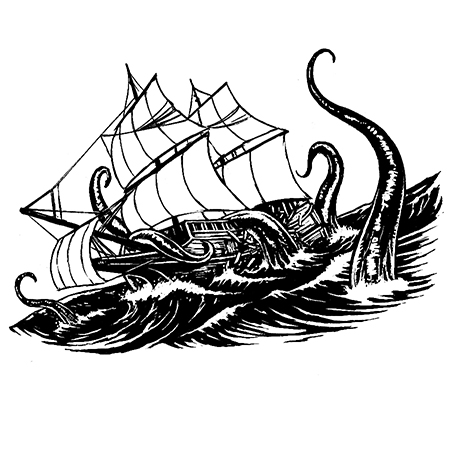
\includegraphics[width=0.9\textwidth,height=0.55\textheight,keepaspectratio]{kraken.jpg}\\[1.5cm]Mystic
of Storms}
  \author{Class Handbook}
\date{}
\maketitle


\clearpage
\thispagestyle{empty}
\begin{center}
\vspace*{\fill}
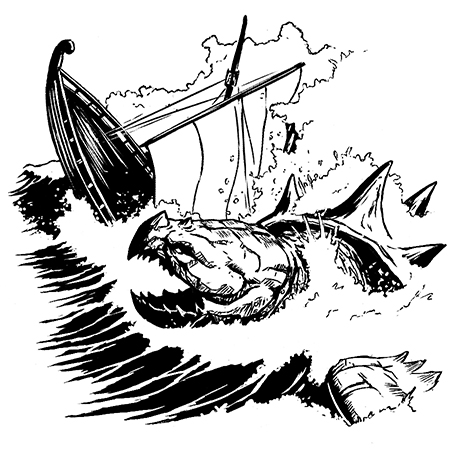
\includegraphics[width=\textwidth,height=0.85\textheight,keepaspectratio]{seaMonster.jpg}\par
\vspace{0.4cm}
{\itshape The fiercest storms are often at sea\ldots{} with a giant
monster too.}\par
\vspace*{\fill}
\end{center}

\clearpage
\twocolumn

\section{Mystic (Storm)}\label{mystic-storm}

\subsection{Core Mystic (Storm) Traits}\label{core-mystic-storm-traits}

\needspace{11\baselineskip}

{\def\LTcaptype{none} % do not increment counter
\begin{table}[!htbp]
\centering
\begin{tabular}{@{}
  >{\raggedright\arraybackslash}p{(\linewidth - 2\tabcolsep) * \real{0.4194}}
  >{\raggedright\arraybackslash}p{(\linewidth - 2\tabcolsep) * \real{0.5806}}@{}}
\toprule\noalign{}
\begin{minipage}[b]{\linewidth}\raggedright
\textbf{Primary Ability}
\end{minipage} & \begin{minipage}[b]{\linewidth}\raggedright
Charisma
\end{minipage} \\
\midrule\noalign{}
\textbf{Hit Points} & 1d6 \\
\textbf{Saving Throw Proficiencies} & Constitution, Charisma \\
\textbf{Skill Proficiencies} & Choose 2 skills \\
\textbf{Weapon Proficiencies} & Choose 3 categories \\
\textbf{Starting Equipment} & Chain Mail, Spear, Longsword, Shield \\
\bottomrule\noalign{}
\end{tabular}
\end{table}
}

\subsection{Mystic (Storm) Features}\label{mystic-storm-features}

\needspace{20\baselineskip}

{\def\LTcaptype{none} % do not increment counter
\begin{table}[!htbp]
\centering
\begin{tabular}{@{}
  >{\raggedright\arraybackslash}p{(\linewidth - 4\tabcolsep) * \real{0.1136}}
  >{\raggedright\arraybackslash}p{(\linewidth - 4\tabcolsep) * \real{0.2500}}
  >{\raggedright\arraybackslash}p{(\linewidth - 4\tabcolsep) * \real{0.6364}}@{}}
\toprule\noalign{}
\begin{minipage}[b]{\linewidth}\raggedright
Level
\end{minipage} & \begin{minipage}[b]{\linewidth}\raggedright
Proficiency
\end{minipage} & \begin{minipage}[b]{\linewidth}\raggedright
Class Features
\end{minipage} \\
\midrule\noalign{}
1 & +2 & Spellcasting, Storm's Fury \\
2 & +2 & --- \\
3 & +2 & Ability Bonus \\
4 & +2 & --- \\
5 & +2 & Storm's Calm \\
6 & +2 & --- \\
7 & +2 & Ability Bonus \\
8 & +2 & --- \\
9 & +3 & Storm's Wrath \\
10 & +3 & --- \\
\bottomrule\noalign{}
\end{tabular}
\end{table}
}

\subsection{Level 1: Spellcasting}\label{level-1-spellcasting}

You can cast spells from the Mystic (Storm) spell list. Charisma is your
casting ability. You know two cantrips.

You prepare a number of spells equal to your total number of spell
slots. You may change your prepared spells after an extended period of
downtime.

You regain all expended spell slots when you finish a long rest. Once
per day, you may regain 1 expended spell slot when you finish a short
rest.

\subsection{Spell Slots by Level}\label{spell-slots-by-level}

\needspace{20\baselineskip}

{\def\LTcaptype{none} % do not increment counter
\begin{table}[!htbp]
\centering
\begin{tabular}{@{}
  >{\raggedright\arraybackslash}p{(\linewidth - 6\tabcolsep) * \real{0.3571}}
  >{\raggedright\arraybackslash}p{(\linewidth - 6\tabcolsep) * \real{0.2143}}
  >{\raggedright\arraybackslash}p{(\linewidth - 6\tabcolsep) * \real{0.2143}}
  >{\raggedright\arraybackslash}p{(\linewidth - 6\tabcolsep) * \real{0.2143}}@{}}
\toprule\noalign{}
\begin{minipage}[b]{\linewidth}\raggedright
Level
\end{minipage} & \begin{minipage}[b]{\linewidth}\raggedright
1
\end{minipage} & \begin{minipage}[b]{\linewidth}\raggedright
2
\end{minipage} & \begin{minipage}[b]{\linewidth}\raggedright
3
\end{minipage} \\
\midrule\noalign{}
1 & 2 & -- & -- \\
2 & 2 & -- & -- \\
3 & 3 & -- & -- \\
4 & 3 & -- & -- \\
5 & 4 & 2 & -- \\
6 & 4 & 2 & -- \\
7 & 4 & 3 & -- \\
8 & 4 & 3 & -- \\
9 & 4 & 3 & 2 \\
10 & 4 & 3 & 2 \\
\bottomrule\noalign{}
\end{tabular}
\end{table}
}

\subsection{Level 1: Storm's Fury}\label{level-1-storms-fury}

Whenever a creature is within 5 feet of you, you can deal 1d8 lightning
damage to the creature. Once you deal damage in this way, you cannot do
so again until the start of your next turn.

The damage increases to 2d8 at level 9.

\subsection{Level 3: Ability Bonus}\label{level-3-ability-bonus}

You gain a +1 bonus to two different abilities of your choice.

\subsection{Level 5: Storm's Calm}\label{level-5-storms-calm}

You gain Resistance to lightning and thunder damage.

\subsection{Level 7: Ability Bonus}\label{level-7-ability-bonus}

You gain a +1 bonus to two different abilities of your choice.

\subsection{Level 9: Storm's Wrath}\label{level-9-storms-wrath}

When you roll lightning or thunder damage, you can deal maximum damage
instead of rolling. You take a failed death save when you use this
feature.

\section{Mystic (Storm) Spells}\label{mystic-storm-spells}

The tables are numbered for random spell selection.

\subsection{Cantrips}\label{cantrips}

\needspace{9\baselineskip}

{\def\LTcaptype{none} % do not increment counter
\begin{table}[!htbp]
\centering
\begin{tabular}{@{}
  >{\raggedright\arraybackslash}p{(\linewidth - 2\tabcolsep) * \real{0.2000}}
  >{\raggedright\arraybackslash}p{(\linewidth - 2\tabcolsep) * \real{0.8000}}@{}}
\toprule\noalign{}
\begin{minipage}[b]{\linewidth}\raggedright
d4
\end{minipage} & \begin{minipage}[b]{\linewidth}\raggedright
Cantrip
\end{minipage} \\
\midrule\noalign{}
1 & Sparks \\
2 & Light \\
3 & Ray of Frost \\
4 & Thaumaturgy \\
\bottomrule\noalign{}
\end{tabular}
\end{table}
}

\subsection{Level 1 Spells}\label{level-1-spells}

\needspace{9\baselineskip}

{\def\LTcaptype{none} % do not increment counter
\begin{table}[!htbp]
\centering
\begin{tabular}{@{}
  >{\raggedright\arraybackslash}p{(\linewidth - 2\tabcolsep) * \real{0.2000}}
  >{\raggedright\arraybackslash}p{(\linewidth - 2\tabcolsep) * \real{0.8000}}@{}}
\toprule\noalign{}
\begin{minipage}[b]{\linewidth}\raggedright
d4
\end{minipage} & \begin{minipage}[b]{\linewidth}\raggedright
Level 1
\end{minipage} \\
\midrule\noalign{}
1 & Bless \\
2 & Feather Fall \\
3 & Thunderwave \\
4 & Wall of Fog \\
\bottomrule\noalign{}
\end{tabular}
\end{table}
}

\subsection{Level 2 Spells}\label{level-2-spells}

\needspace{9\baselineskip}

{\def\LTcaptype{none} % do not increment counter
\begin{table}[!htbp]
\centering
\begin{tabular}{@{}
  >{\raggedright\arraybackslash}p{(\linewidth - 2\tabcolsep) * \real{0.1579}}
  >{\raggedright\arraybackslash}p{(\linewidth - 2\tabcolsep) * \real{0.8421}}@{}}
\toprule\noalign{}
\begin{minipage}[b]{\linewidth}\raggedright
d4
\end{minipage} & \begin{minipage}[b]{\linewidth}\raggedright
Level 2
\end{minipage} \\
\midrule\noalign{}
1 & Levitate \\
2 & Misty Step \\
3 & Silence \\
4 & See Invisibility \\
\bottomrule\noalign{}
\end{tabular}
\end{table}
}

\subsection{Level 3 Spells}\label{level-3-spells}

\needspace{9\baselineskip}

{\def\LTcaptype{none} % do not increment counter
\begin{table}[!htbp]
\centering
\begin{tabular}{@{}
  >{\raggedright\arraybackslash}p{(\linewidth - 2\tabcolsep) * \real{0.1667}}
  >{\raggedright\arraybackslash}p{(\linewidth - 2\tabcolsep) * \real{0.8333}}@{}}
\toprule\noalign{}
\begin{minipage}[b]{\linewidth}\raggedright
d4
\end{minipage} & \begin{minipage}[b]{\linewidth}\raggedright
Level 3
\end{minipage} \\
\midrule\noalign{}
1 & Fly \\
2 & Haste \\
3 & Lightning Bolt \\
4 & Water Breathing \\
\bottomrule\noalign{}
\end{tabular}
\end{table}
}

\section{Mystic (Storm) Spell List}\label{mystic-storm-spell-list}

Spells descriptions are listed below.

\subsection{Bless}\label{bless}

\textbf{Level:} 1

\textbf{Range:} 30 feet

\textbf{Duration:} Concentration, up to 1 minute

You bless up to three creatures within range. A blessed creature adds
1d4 to their attack rolls and saves.

\subsection{Feather Fall}\label{feather-fall}

\textbf{Level:} 1

\textbf{Range:} 60 feet

\textbf{Duration:} 1 minute

You can cast this spell in response to falling or seeing someone fall.
Choose up to five falling creatures within range. A falling creature's
rate of descent slows to 60 feet per round. If a creature lands before
the spell ends, the creature takes no damage from the fall, and the
spell ends for that creature.

\subsection{Fly}\label{fly}

\textbf{Level:} 3

\textbf{Range:} Touch

\textbf{Duration:} Concentration, up to 10 minutes

You touch a willing creature. For the duration, the target gains a fly
speed.

When the spell ends, the target falls if it is still aloft unless it can
stop the fall.

\subsection{Haste}\label{haste}

\textbf{Level:} 3

\textbf{Range:} 30 feet

\textbf{Duration:} Concentration, up to 1 minute

Choose a willing creature within range. On each of its turns, it can
choose to take a second action. If it does so, roll a d20. On an 11 or
higher, it gains a failed death save.

\subsection{Levitate}\label{levitate}

\textbf{Level:} 2

\textbf{Range:} 60 feet

\textbf{Duration:} Concentration, up to 10 minutes

One creature or loose object of your choice within range rises
vertically up to 20 feet and remains suspended there. The spell can
levitate an object that weighs up to 500 pounds. An unwilling creature
that succeeds on a Constitution saving throw is unaffected.

The target can move only by pushing or pulling against a fixed object or
surface within reach (such as a wall or a ceiling), which allows it to
move as if it were climbing. You can change the target's altitude by up
to 20 feet in either direction on your turn. If you are the target, you
can move up or down as part of your move. Otherwise, you can take an
action to move the target, which must remain within the spell's range.

When the spell ends, the target floats gently to the ground if it is
still aloft.

\subsection{Light}\label{light}

\textbf{Level:} Cantrip

\textbf{Range:} Touch

\textbf{Duration:} 1 hour

An object you touch sheds dim light in a 30-foot radius and Dim Light
for an additional 20 feet. The spell ends if you cast it again.

\subsection{Lightning Bolt}\label{lightning-bolt}

\textbf{Level:} 3

\textbf{Range:} 300 feet

You can make ranged spell attacks against up to three targets. The
damage is 6d10 lightning damage if you attack three targets, 8d10
lightning damage if you attack two, or 10d10 lightning damage if you
attack one. If the attack misses, the target takes half damage.

\subsection{Misty Step}\label{misty-step}

\textbf{Level:} 2

\textbf{Range:} Self

Briefly surrounded by silvery mist, you teleport up to 30 feet to an
unoccupied space you can see. Casting this spell does not use your
action.

\newpage

\subsection{Ray of Frost}\label{ray-of-frost}

\textbf{Level:} Cantrip

\textbf{Range:} 60 feet

A frigid beam of blue-white light streaks toward a creature within
range. Make a ranged spell attack against the target. On a hit, it takes
1d8 cold damage, and its speed is reduced by 20 feet until after its
next turn.

The damage increases to 2d8 cold damage at level 5 and 3d8 cold damage
at level 9.

\subsection{See Invisibility}\label{see-invisibility}

\textbf{Level:} 2

\textbf{Range:} Self

\textbf{Duration:} 1 hour

You see creatures and objects that are invisible as if they were
visible.

\subsection{Silence}\label{silence}

\textbf{Level:} 2

\textbf{Range:} 120 feet

\textbf{Duration:} Concentration, up to 10 minutes

No sound can be created within or pass through a 20-foot-radius sphere
centered on a point you choose within range. Any creature or object
entirely inside the sphere has immunity to thunder damage. Spells cannot
be cast in the spell's area.

\newpage

\subsection{Sparks}\label{sparks}

\textbf{Level:} Cantrip

\textbf{Range:} 120 feet

You send a bolt of scintillating lightning energy at a foe. Make a
ranged attack against the target. On a hit, the target takes 1d6
lightning damage and falls prone.

The damage increases to 2d6 lightning damage at level 5 and 3d6
lightning damage at level 9.

\subsection{Thaumaturgy}\label{thaumaturgy}

\textbf{Level:} Cantrip

\textbf{Range:} 30 feet

\textbf{Duration:} Up to 1 minute

You manifest a minor wonder within range. You can create minor
illusions, alter one of your physical traits, change the sound or volume
of your voice, and otherwise make cosmetic changes to yourself or an
object in range. The spell ends if you cast it again.

\newpage

\subsection{Thunderwave}\label{thunderwave}

\textbf{Level:} 1

\textbf{Range:} Self

You unleash a wave of thunderous energy. Each creature in a 15-foot cube
originating from you makes a Constitution saving throw. On a failed
save, a creature takes 2d8 thunder damage and is pushed 10 feet away
from you. On a successful save, a creature takes half damage.

Unsecured objects that are entirely within the cube are pushed 10 feet
away from you, and a thunderous boom is audible within 300 feet.

The damage increases to 3d8 thunder damage if you use a level 2 slot and
4d8 thunder damage if you use a level 3 slot.

\subsection{Wall of Fog}\label{wall-of-fog}

\textbf{Level:} 1

\textbf{Range:} 120 feet

\textbf{Duration:} 10 minutes

You create a thick, billowing wall of fog that blocks sight and sound.
It is one-foot thick, 10 feet high, and up to 30 feet long. The wall can
bend and turn as you wish, but all of it must be within the spell's
range when you create it.

\subsection{Water Breathing}\label{water-breathing}

\textbf{Level:} 3

\textbf{Range:} 30 feet

\textbf{Duration:} 24 hours

This spell grants up to ten willing creatures of your choice within
range the ability to breathe underwater until the spell ends. Affected
creatures also retain their normal mode of respiration.

\newpage

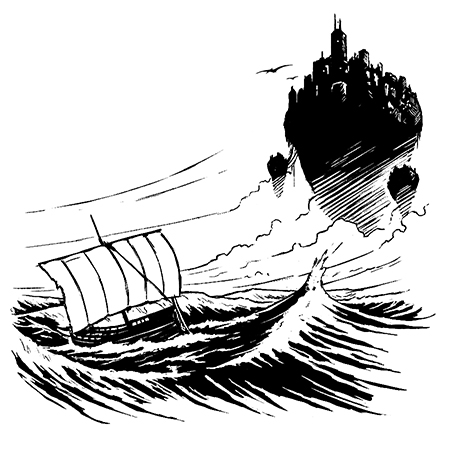
\includegraphics[width=1\linewidth,height=\textheight,keepaspectratio]{bigWave.jpg}

\onecolumn

\clearpage
\thispagestyle{empty}
\begin{center}
\vspace*{\fill}
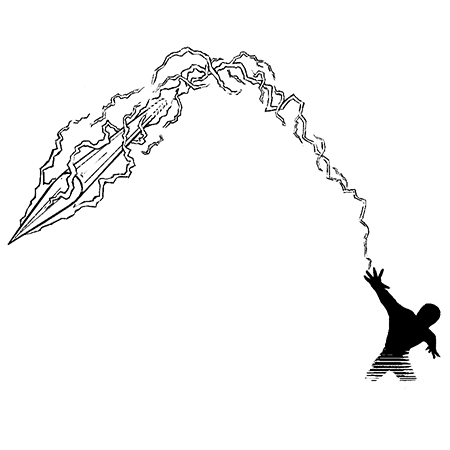
\includegraphics[width=0.7\textwidth,keepaspectratio]{lightningArrow.jpg}\par
\vspace{0.4cm}
{\itshape Lightning is power incarnate, straight from the heavens.}\par
\vspace*{\fill}
\end{center}

\end{document}